\documentclass[11pt,a4paper]{report}
\usepackage{fullpage}
\usepackage{amsmath}
\usepackage{graphicx}
\usepackage{caption}
\usepackage[authoryear,round]{natbib}

\usepackage[margin=2.5cm,top=1cm,bottom=1cm]{geometry}
\setlength{\parindent}{0pt}
\pagenumbering{gobble}

\begin{document}

\begin{center}
	\begin{minipage}[b]{0.5\linewidth}
	\centering
	
\includegraphics[width=0.4\linewidth]{Hybrid_tree2.eps}\\
	\captionof{figure}{Species tree $S$. B is a hybrid, having ancestry
		from both A and C lineages, with proportion $\gamma$ coming
		from the A lineage. $t$ represents the time between
		the top of the tree and the hybridisation event.}
	\end{minipage}
\end{center}
	%\vspace{4mm}

	\begin{minipage}[b]{0.3\linewidth}
		\centering
		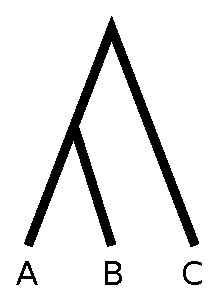
\includegraphics[width=0.66\linewidth]{Hybrid_tree_ab.eps}\\
		\captionof{figure}{Species tree $S_1$. Genes belong to this tree with probability $\gamma$.}
		\begin{align*}
p(ab|S_1, t) &= 1 - \frac{2}{3}e^{-t}\\
p(bc|S_1, t) &= \frac{1}{3}e^{-t}\\
p(ac|S_1, t) &= \frac{1}{3}e^{-t}\\
\end{align*}

	\end{minipage}
	\hfill
	\begin{minipage}[b]{0.3\linewidth}
		\centering
		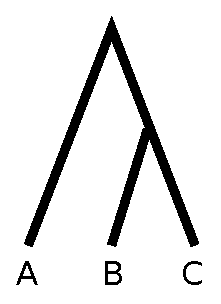
\includegraphics[width=0.66\linewidth]{Hybrid_tree_bc.eps}
		\captionof{figure}{Species tree $S_2$. Genes belong to this tree with probability $1-\gamma$.}
		\begin{align*}
p(ab|S_2, t) &= \frac{1}{3}e^{-t}\\
p(bc|S_2, t) &= 1 - \frac{2}{3}e^{-t}\\
p(ac|S_2, t) &= \frac{1}{3}e^{-t}\\
\end{align*}

	\end{minipage}

%\begin{align*}
%p(ab|S_1, t) &= 1 - \frac{2}{3}e^{-t}\\
%p(bc|S_1, t) &= \frac{1}{3}e^{-t}\\
%p(ac|S_1, t) &= \frac{1}{3}e^{-t}\\
%p(ab|S_2, t) &= \frac{1}{3}e^{-t}\\
%p(bc|S_2, t) &= 1 - \frac{2}{3}e^{-t}\\
%p(ac|S_2, t) &= \frac{1}{3}e^{-t}\\
%\end{align*}

$p(ab|S_1, t)$ gives the probability of observing that A and B coalesce most recently,
given species tree $S_1$ and time $t$ between first and second coalescent
events \citep{meng_detecting_2009}.
Other probabilities are defined similarly.
For $n$ independent gene trees (from SNPs in our case),
we bin each locus into one of the gene trees $ab$, $bc$, or $ac$,
according to the putative most recent coalescent event.
Given counts of the putative gene trees, $g = \{n_{ab},n_{bc},n_{ac}\}$, we
calculate the joint likelihood of $\gamma$ and $t$.


\begin{align*}
L(\gamma,t|S,g) &= [\gamma{}p(ab|S_1,t) + (1-\gamma)p(ab|S_2,t)]^{n_{ab}}\\
		& \cdot [\gamma{}p(bc|S_1,t) + (1-\gamma)p(bc|S_2,t)]^{n_{bc}}\\
		& \cdot [\gamma{}p(ac|S_1,t) + (1-\gamma)p(ac|S_2,t)]^{n_{ac}}\\
 &= (\gamma + \frac{1}{3}e^{-t} - \gamma{}e^{-t})^{n_{ab}}
	(1-\gamma-\frac{2}{3}e^{-t} + \gamma{}e^{-t})^{n_{bc}}
	(\frac{1}{3}e^{-t})^{n_{ac}}\\
log(L) &= n_{ab}log(\gamma + \frac{1}{3}e^{-t} - \gamma{}e^{-t})
	+ n_{bc}log(1-\gamma-\frac{2}{3}e^{-t} + \gamma{}e^{-t})
	+ n_{ac}(log(\frac{1}{3}) -t)
\end{align*}

\pagebreak
\bibliographystyle{PLoS-Biology}
\bibliography{refs}

\end{document}
